\documentclass[a4paper, 11pt, oneside]{scrbook}

\usepackage[backend=biber]{biblatex}
\usepackage[ngerman]{babel}		
\usepackage[T1]{fontenc}	  	
\usepackage[utf8]{inputenc}
\usepackage[hidelinks]{hyperref}
\usepackage{graphicx}
\usepackage{epstopdf}
\usepackage{float}
\usepackage{microtype}
\usepackage[T1]{fontenc}
\usepackage{lmodern}
\usepackage{acronym}
\usepackage{booktabs}
\usepackage{caption}
\usepackage{csquotes}
\usepackage{url}
\usepackage{makecell}
\usepackage[table]{xcolor}
\usepackage{listings}
\usepackage{pdfpages}
\usepackage{siunitx}


% \usepackage{blindtext}

\renewcommand*{\headfont}{\normalfont}
\renewcommand*{\multicitedelim}{\addsemicolon\space}
% \renewcommand*{\headrulewidth}{0pt}
\renewcommand*{\arraystretch}{1.5}
\renewcommand*{\familydefault}{\sfdefault}

\newcommand*{\tabindent}{\hspace{3mm}}
\newcommand*{\doubletabindent}{\hspace{6mm}}

\setlength{\parskip}{1.5ex}
\lstset{numbers=left, numberstyle=\tiny, numbersep=5pt, firstnumber=1}
\lstset{language=Perl, basicstyle=\ttfamily\footnotesize,breaklines=true}

\addbibresource{bibliography.bib}
\counterwithin{figure}{section}

\begin{document} 

\rowcolors{1}{white}{lightgray}

\frontmatter

\def\title{Elephant Herding Optimization}
\def\author{Robin Wollenschläger}

\begin{titlepage}


    \begin{minipage}[t]{0.25\textwidth}
        DHBW Mosbach\\
        Lohrtalweg 10\\
        74821 Mosbach\\
        Deutschland
    \end{minipage}
    \hfill
    \begin{minipage}[t]{0.25\textwidth}
        
\includegraphics[height=1.5cm]{prefix/image/logo-dhbw.eps}
    \end{minipage}




    \begin{center}
        \vspace{10mm}

        \huge \title

        \vspace{5mm}

        \large \bfseries Studienarbeit EMIT an der Dualen Hochschule Baden-Württemberg Mosbach


    \end{center}

    \vspace{10mm}

    \begin{tabular}[ht]{ l p{4cm} l p{4cm} }
        Studiengang/-richtung:                               & B.Sc. - Angewandte Informatik  \tabularnewline
        Kurs:                                                & INF20B\tabularnewline
        Name, Vorname:                                       & \author \tabularnewline
        Name, Vorname des wiss. Prüfenden/Betreuenden:       & Prof. Dr. Carsten Müller \tabularnewline
    \end{tabular}

    % \chapter*{Sperrvermerk}
    % \thispagestyle{empty}
    % Der Inhalt dieser Arbeit darf weder als Ganzes noch in Auszügen Personen außerhalb des Prüfungsprozesses und des  Evaluationsverfahrens zugänglich gemacht werden, sofern keine anders lautende Genehmigung der Ausbildungsstätte vorliegt.

    % \chapter*{Anmerkung Bilder/Screenshots}
    % Bilder und Screenshots in dieser Arbeit wurden bewusst ohne Daten erstellt, um den datenschutzrechtlichen Bestimmungen zu entsprechen. Falls dies nicht möglich war, wurden Bereiche mit personenbezogenen Daten geschwärzt.

    % \chapter*{Ehrenw\"ortliche Erkl\"arung}

    % \thispagestyle{empty}
    % Ich versichere hiermit, dass ich diese Arbeit selbstständig verfasst und keine anderen als die angegebenen Quellen und Hilfsmittel benutzt habe. \\
    % Ich versichere zudem, dass die eingereichte elektronische Fassung mit der gedruckten Fassung übereinstimmt.\\
    % \\
    % Buchen, \today
    % \newpage
    % \vspace{5mm}

    % \fancypagestyle{empty}{
    %   \fancyhf{}
    %   \fancyfoot[C]{\today}
    % }

\end{titlepage}


% \chapter*{Abkürzungsverzeichnis}
\begin{acronym}[.NET-Framework]
    \acro{SPS}[SPS]{Speicherprogrammierbare Steuerung}
\end{acronym}  

% \listoffigures

% \listoftables
 
\tableofcontents

\mainmatter

\chapter{Einleitung}

\section{Optimierungsalgorithmen aus dem Bereich der Schwarmintelligenz}
Algorithmen aus dem Bereich der Schwarmintelligenz werden zur Optimierung von Problemen verwendet, in dem Verhaltensstrukturen aus der Natur mathematisch abgebildet und nutzbar gemacht werden.\\
Dabei wird versucht im Verhalten von Lebewesen Muster zu finden, mit denen ein Ziel erreicht werden kann, um somit die Zielfindung mathematischer Probleme zu optimieren. Gesucht wird dabei ein Optimum, also ein globales Minimum oder Maximum einer mehrdimensionalen mathematischen Funktion.\\
Der Algorithmus 'Grey Wolf Optimization' arbeitet rundenbasiert in Iterationen, wobei eine Obergrenze definiert werden kann.

\section{Grauwölfe}
\subsection{Sozialverhalten}
Grauwölfe (Canis lupus) leben in Rudeln mit einer festen Hierarchie, die sich in Alpha-, Beta-, Delta- und Omega-Wölfe gliedert (siehe \autoref{gwo_hierarchy}). \\
Pro Rudel gibt es jeweils  Alpha-, Beta- und Deltawölfe. Der Rest des Rudels wird als Omegawolf klassifiziert. Diese Hierarchie ist sehr strikt und das Rudel folgt meist den Entscheidungen des Anführers (Alpha), auch wenn es selten zu demokratischen Entscheidungen kommen kann und der Alpha den anderen Mitgliedern des Rudels folgt. Der Alpha muss dabei nicht zwingend das stärkste Tier des Rudels sein, sondern der beste Anführer, der die besten Entscheidungen trifft. \\
Die zweite Hierarchieebene innerhalb des Rudels wird vom Betawolf eingenommen. Er hilft dem Alpha bei der Entscheidungsfindung und hat im Falle eines Dahinscheidens des Alpha die besten Chancen seinen Platz als Nachfolger und neuer Anführer des Rudels einzunehmen. Innerhalb des Rudels setzt der Beta die Anweisungen des Alpha durch und sorgt für Disziplin und Ordnung unter den niederrangigen Wölfen.\\
Diese niederrangigen Mitglieder sind aufgeteilt in Delta- und Omegawölfe. Der Delta muss zwar den Anweisungen von Alpha und Beta Folge leisten, dominiert aber über die Omegawölfe und fungiert in Rollen wie Scout, Wächter oder Jäger und tragen damit Sorge über die Sicherheit des Rudels und des zugehörigen Territoriums oder es handelt sich um Ältere, die zuvor den Rang eines Alpha oder Beta bekleidet haben.\\
Omegawölfe sind die Rangniedersten innerhalb des Rudels, aber sie sind für die soziale Struktur dennoch sehr wichtig, da es beim Verlust eines Omegas zu Kämpfen und Problemen innerhalb des Rudels kommt und die Hierarchie wieder hergestellt werden muss. Die Dominanz über die Omegas dient den anderen Wölfen zum Teil als Ventil und sorgt so dafür, dass sich innerhalb des Rudels keine Aggressionen anstauen, \cite[vgl. Mirjalili 2014, S.4f]{MIRJALILI201446}.\\

\begin{figure}[ht]
    \begin{center}
        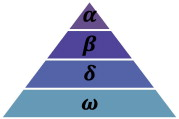
\includegraphics[width=0.4\textwidth]{assets/img/Grey_wolf_social_hierarchy.jpg}
        \caption[Soziale Hierarchie bei Grauwölfen]{Soziale Hierarchie bei Grauwölfen \cite{MIRJALILI201446}}
        \label{gwo_hierarchy}
    \end{center}
\end{figure}

\subsection{Jagdverhalten}
Neben dem Sozialverhalten ist das Jagdverhalten der Grauwölfe von besonderem Interesse. Dieses teilt sich nach \cite[vgl. Mirjalili 2014, S.5]{MIRJALILI201446} in folgende Phasen: 
\begin{itemize}
    \item Suchen, Jagen und Erreichen der Beute
    \item Verfolgen, Einkreisen und Beunruhigen der Beute, bis sie stehen bleibt
    \item Angreifen der Beute 
\end{itemize}
% \begin{figure}[ht]
%     \begin{center}
%         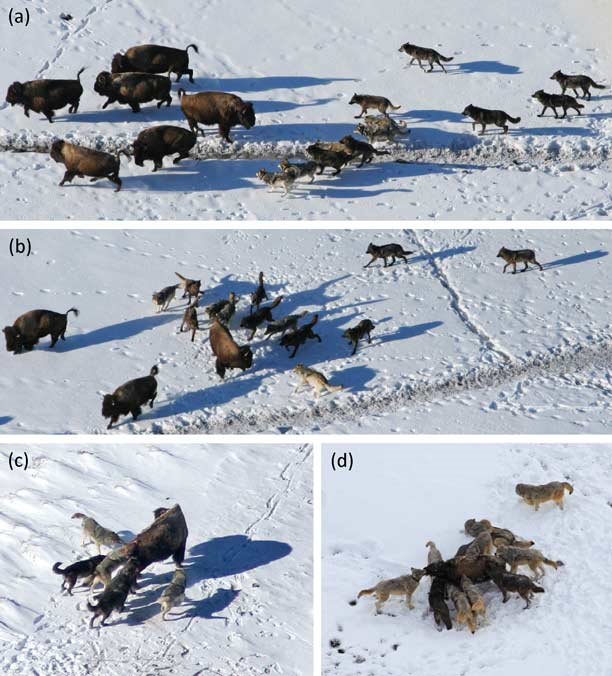
\includegraphics[width=0.9\textwidth]{assets/img/wolf-hunt-study_plos_612x676.png}
%         \caption[Jagdverhalten bei Grauwölfen]{Jagdverhalten bei Grauwölfen \cite{yellowstoneparkWolfhunt}}
%         \label{gwo_hunt}
%     \end{center}
% \end{figure}
% Diese Phasen sind in \autoref{gwo_hunt} dargestellt.\\
Der Algorithmus 'Grey Wolf Optimization' stützt sich auf die mathematische Umsetzung des Jagdverhaltens und des Sozialverhaltens von Grauwölfen.

{\let\clearpage\relax \chapter{Optimierung}}
\section{Initialisierung}
Zu Beginn muss die Herde aller Elefanten in Clans aufgeteilt werden, wobei davon ausgegangen wird, dass jeder Clan eine feste Nummer an Tieren beinhaltet, genau einen Matriarchen hat und, dass mit jeder Generation eine feste Anzahl an männlichen Elefanten ihren Clan verlässt, \cite[vgl. Wang et al, S.2]{wang_deb_coelho_2015}. 

\section{Clan-Update-Operator} \label{eho_clanUpdate}
Jeder Clan hat einen Matriarchen, dem die Tiere folgen. Daher ist die neue Position $x_{new, ci, j}$ eines Elefanten $j$ in Abhängigkeit von seinem Clan $ci$ und der Position des zugehörigen Matriarchen $x_{best, ci}$ bestimmt (siehe \autoref{calcXNew}). 
\begin{equation}
    x_{new, ci, j} + \alpha \cdot (x_{best, ci} - x_{ci, j}) \cdot r
    \label{calcXNew}
\end{equation}
$x_{ci, j}$ stellt dabei die alte Position des Elefanten und $\alpha \in [0,1]$ einen Skalierungsfaktor, der den Einfluss des Matriarchen ausdrückt. Für $r$ gilt $r \in [0,1]$.\\
\\
Die Position des Matriarchen kann mit \autoref{calcXNew} nicht berechnet werden und es muss \autoref{calcXNewMatriarch} genutzt werden.
\begin{equation}
    x_{new, ci, j} = \beta \cdot x_{center, ci}
    \label{calcXNewMatriarch}
\end{equation}
Die Position des Matriarchen wird mittels der Position des zentralen Tieres $x_{center, ci}$ innerhalb des Clans $ci$ und $\beta \in [0,1]$ repräsentiert einen Skalierungsfaktor. $x_{center, ci}$ kann mittels \autoref{calcXCenter} berechnet werden.
\begin{equation}
    x_{center, ci, d} = \frac{1}{n_{ci}} \cdot \sum_{j=1}^{n_{ci}} x_{ci,j,d}
    \label{calcXCenter}
\end{equation}
Die Position des Tieres $x_{center, ci}$ ist zusätzlich abhängig von der Dimension $d$ mit $1 \leq d \leq D$ und der Anzahl der Tiere in einem Clan $n_{ci}$, \cite[vgl. Wang et al, S.2]{wang_deb_coelho_2015}.

\section{Separierungs-Operator} \label{eho_separate}
Der Separierungsprozess beschreibt das Verlassen der männlichen Elefanten des Clans beim Heranwachsen. Die Zahl der Mitglieder bleibt dabei jedoch gleich, die Elefanten werden lediglich ersetzt. Zur Optimierung der Annäherung an das Ziel wird dabei angenommen, dass der Elefant mit der schlechtesten Position ($x_{worst, ci}$) zum Ziel den Clan verlässt (siehe \autoref{calcXWorst}).
\begin{equation}
    x_{worst, ci} = x_{min} + (x_{max} - x_{min} + 1) \cdot rand
    \label{calcXWorst}
\end{equation}
$x_{max}$ und $x_{min}$ stellen die oberen bzw. unteren Grenzen der jeweiligen Dimension dar und $rand \in [0,1]$ eine Zufallszahl, \cite[vgl. Wang et al, S.2]{wang_deb_coelho_2015}.

\section{Algorithmus}
\begin{figure}[ht]
    \begin{center}
        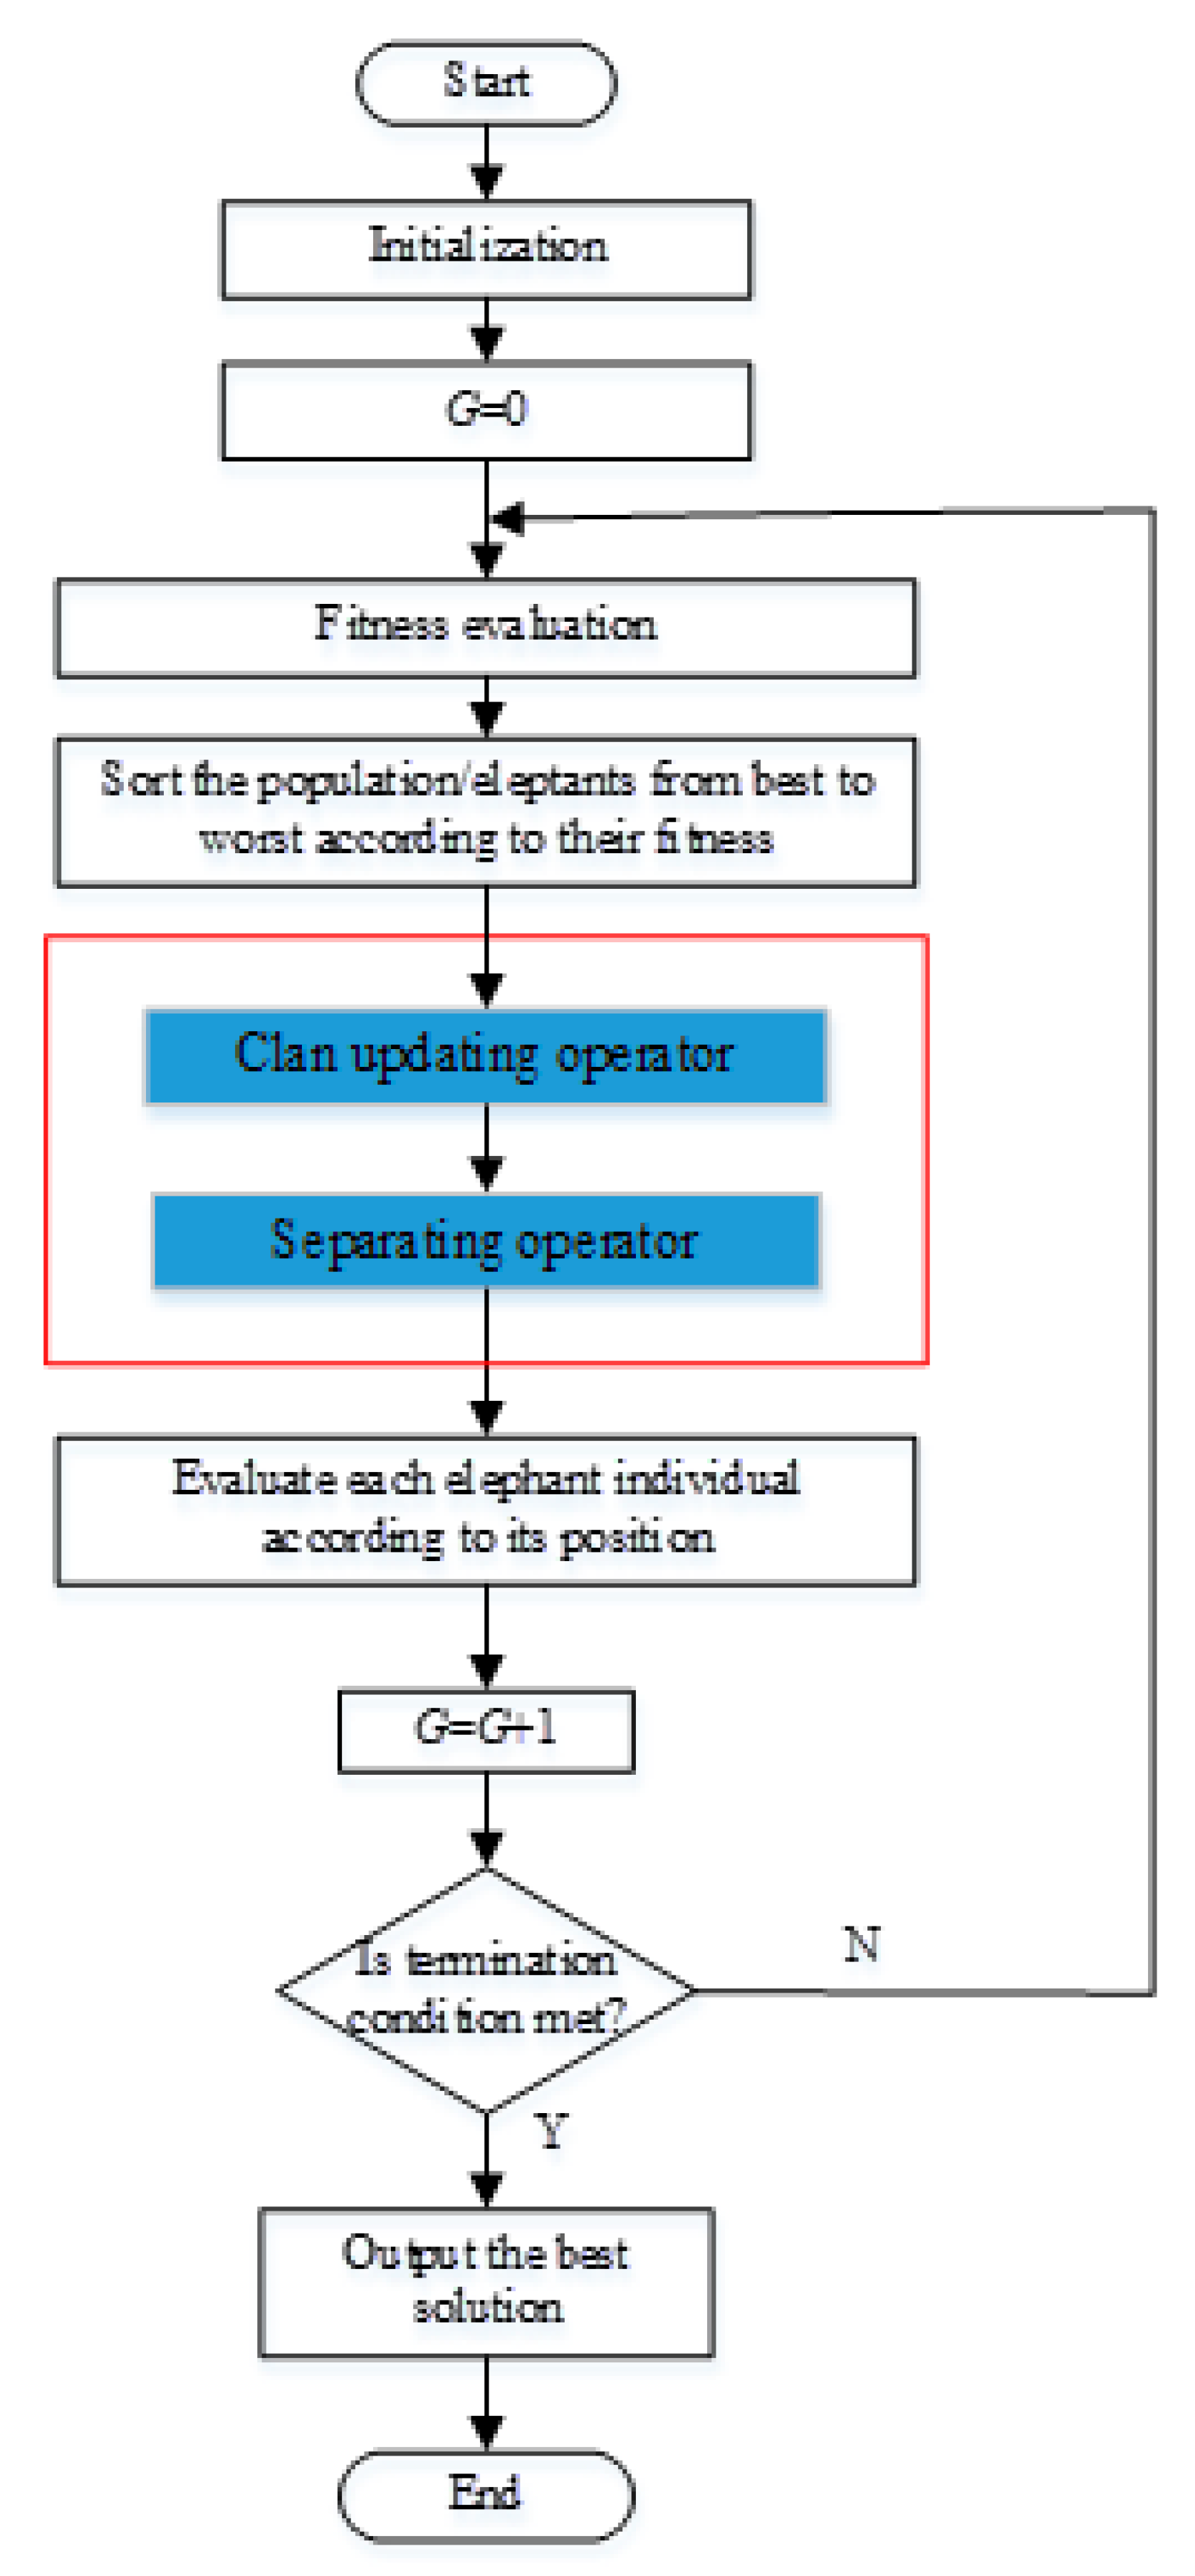
\includegraphics[width=0.3\textwidth]{assets/img/eho_flowchart.png}
        \caption[EHO Flowchart]{\cite[Li et al, S.4]{li_lei_alavi_wang_2020}}
        \label{eho_flowchart}
    \end{center}
\end{figure}
Aus \autoref{eho_clanUpdate} und \autoref{eho_separate} ergibt sich der Ablauf \autoref{eho_flowchart}, der aufzeigt, dass über die Generationen die einzelnen Elefanten immer näher hin zum gesuchten Optimum konvergieren, bis das Endkriterium erreicht ist. Dieses wird durch die maximale Anzahl an Generationen definiert.\\
In \autoref{eho_pseudocode} ist der zugehörige Pseudocode aufgeführt.\\
\begin{figure}[ht]
    \begin{center}
        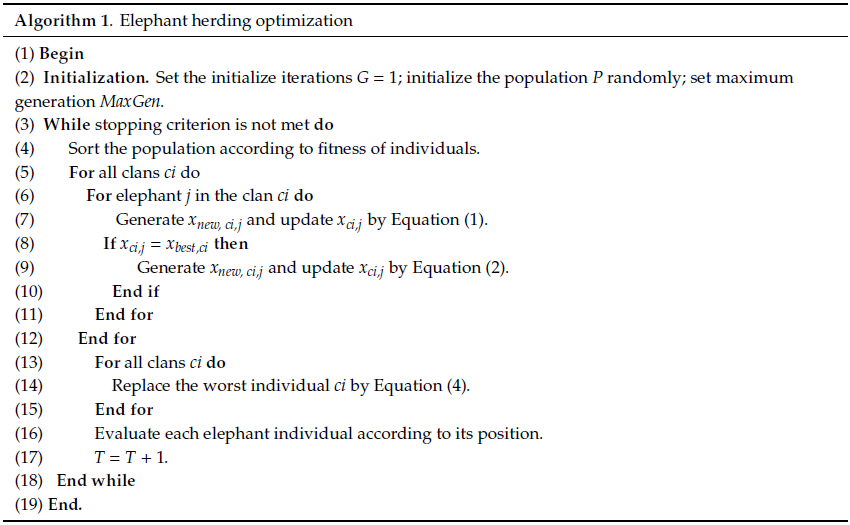
\includegraphics[width=0.7\textwidth]{assets/img/eho_pseudocode.PNG}
        \caption[EHO Pseudocode]{\cite[Li et al, S.5]{li_lei_alavi_wang_2020}}
        \label{eho_pseudocode}
    \end{center}
\end{figure}
Die Elephant Herding Optimization setzt auf eine weitere Unterteilung der Sucher, durch die Aufteilung der Herde in Clans, die als Subgruppen agieren. Dadurch ergibt sich eine höhere Diversität bei der Suche, was zu einer geringeren benötigten Anzahl an Generationen führen kann.\\
Durch die Separierung kann die Konvergenz zum Optimum gezielt erhöht werden, allerdings sollte die Anzahl separierter Tiere nicht höher, als $\frac{n_{ci}}{2}$ liegen, da sonst auch Tiere separiert werden, die zur Zielstrebigkeit des Clans positiv beitragen.  
% \input{chapters/chapter2_Einleitung.tex}
% \input{chapters/chapter3_Planung.tex}
% \input{chapters/chapter4_Durchfuehrung.tex}
% \input{chapters/chapter5_Test.tex}
% \input{chapters/chapter6_Abnahme.tex}
% \input{chapters/chapter7_Auswertung.tex}
% \input{chapters/chapter8_Fazit.tex}

%\blinddocument

% \nocite{*}

% \appendix
% \setcounter{chapter}{23}
\chapter{Anhang}
\pagenumbering{Roman}

% \section{Basis Kapillarrheometer}
% Quelle: GÖTTFERT Werkstoff-Prüfmaschinen GmbH
% \begin{figure}[ht]
%     \begin{center}
%         \includegraphics[width=0.75\textwidth]{assets/img/DE_IMG_Prinzip_Kapillarrheometer.png}
%         \caption{Basis Kapillarrheometer}
%         \label{base_capillary_rheometer}
%     \end{center}
% \end{figure}
% \clearpage

% \section{RHEOGRAPH 50}
% Quelle: GÖTTFERT Werkstoff-Prüfmaschinen GmbH
% \begin{figure}[ht]
%     \begin{center}
%         \includegraphics[width=0.75\textwidth]{assets/img/IMG_RG50_perspektive.png}
%         \caption{RHEOGRAPH 50}
%         \label{rg50}
%     \end{center}
% \end{figure}
% \clearpage

% % \section{Detaillierte Zeitplanung nach Phasen}
% \begin{table}[ht]
%     \begin{center}
%         \begin{tabular}{| l | r  r |}
%             \hline
%             \textbf{Projektphase}                                & \multicolumn{2}{ c |}{\textbf{Zeit in h}}                \\
%             \hline

%             \textbf{Planungsphase}                               &                                           & \textbf{80} \\
%             \hline
%             \tabindent{IST-Analyse}                              & 20                                        &              \\
%             \hline
%             \tabindent{SOLL-Konzept}                             & 20                                        &              \\
%             \hline
%             \tabindent{Ablaufplanung}                            & 20                                        &              \\
%             \hline
%             \tabindent{Zeit- und Ressourcenplanung}              & 20                                        &              \\
%             \hline

%             \textbf{Durchführung}                                &                                           & \textbf{280} \\
%             \hline
%             \tabindent{Automation Mess- und Kalibrierprozess}    &                                           & 160          \\
%             \hline
%             \doubletabindent{Ablauf Temperaturmessung}           & 80                                       &              \\
%             \hline
%             \doubletabindent{Datenspeicherung}                   & 80                                        &              \\
%             \hline
%             \tabindent{Datentransfer und Auswertung}             &                                           & 120          \\
%             \hline
%             \doubletabindent{Datentransfer}                      & 40                                        &              \\
%             \hline
%             \doubletabindent{Integration PowerTool}              & 40                                        &              \\
%             \hline
%             \doubletabindent{Ermittlung Korrekturwert}           & 20                                        &              \\
%             \hline
%             \doubletabindent{Erstellung Prozessprotokoll}        & 20                                        &              \\
%             \hline

%             \textbf{Testphase/Abnahme}                           &                                           & \textbf{40}  \\
%             \hline
%             \tabindent{Testen einzelner Komponenten}             & 16                                        &              \\
%             \hline
%             \tabindent{Testen im Livebetrieb}                    & 16                                         &              \\
%             \hline
%             \tabindent{Abnahme durch Projektteam}                & 8                                        &              \\
%             \hline

%             \textbf{Auswertung/Fazit/Dokumentation}              &                                           & \textbf{80} \\
%             \hline
%             \tabindent{Auswertung: Gewinn durch Automatisierung} & 8                                        &              \\
%             \hline
%             \tabindent{Projekt-Dokumentation}                    & 72                                        &              \\

%             \hline \hline
%             \textbf{Gesamt}                                      &                                           & \textbf{480} \\
%             \hline
%         \end{tabular}
%     \end{center}
%     \caption{Detaillierte Zeitplanung nach Phasen}
%     \label{zeitplanung-detail}
% \end{table}
% \clearpage


% % \section{ISO 11443 2021}
% % % \begin{figure}[ht]
% %     % \begin{center}
% %         \includepdf[pages=-]{assets/pdf/ISO 11443_2021.pdf}
% %         % \includegraphics[width=0.9\textwidth, page=]{assets/pdf/ISO 11443_2021.pdf}
% %         % \caption{ISO 11443 2021}
% %         % \label{iso_11443_2021}
% %     % \end{center}
% % % \end{figure}
% % \clearpage

% \section{Temperaturkalibrierung und -justierung Hauptprozess}
% Quelle: GÖTTFERT Werkstoff-Prüfmaschinen GmbH
% \begin{figure}[ht]
%     \begin{center}
%         \includegraphics[width=1.0\textwidth]{assets/img/Temperaturkalibrierung RG.png}
%         \caption{Temperaturkalibrierung und -justierung BPMN - Hauptprozess}
%         \label{Temperaturkalibrierung_RG_Haupt}
%     \end{center}
% \end{figure}
% \clearpage

% \section{Unterprozess Korrekturwertbestimmung}
% Quelle: GÖTTFERT Werkstoff-Prüfmaschinen GmbH
% \begin{figure}[ht]
%     \begin{center}
%         \includegraphics[width=1.0\textwidth]{assets/img/Korrekturwerte bestimmen.png}
%         \caption{Bestimmung Korrekturwerte BPMN}
%         \label{Temperaturkalibrierung_RG_Sub_Korr}
%     \end{center}
% \end{figure}
% \clearpage

% \section{Unterprozess Temperaturkalibrierung}
% Quelle: GÖTTFERT Werkstoff-Prüfmaschinen GmbH
% \begin{figure}[ht]
%     \begin{center}
%         \includegraphics[width=1.0\textwidth]{assets/img/Temperaturwerte ziehen.png}
%         \caption{Temperaturkalibrierung BPMN}
%         \label{Temperaturkalibrierung_RG_Sub_Temp}
%     \end{center}
% \end{figure}
% \clearpage

% \section{Zeichnung Heißkanal RHEOGRAPH}\label{drawing_chamber_channel}
% Quelle: GÖTTFERT Werkstoff-Prüfmaschinen GmbH
% %  \begin{figure}[ht]
% %     \begin{center}
% \includepdf[pages=-, landscape=true]{assets/pdf/012.06.0.04.628.0_DOKU.pdf}

% %  \includegraphics[width=1.4\textwidth, angle=90]{assets/pdf/012.06.0.04.628.0_DOKU.pdf}
% %  \caption{Zeichnung Heißkanal RHEOGRAPH}

% %     \end{center}
% %  \end{figure}
% \clearpage

% \section{Dostmann P755 externes Temperaturmessgerät}
% Quelle: \href{https://dostmann-electronic.de/gallery/1208gross_p455_p755_log_multifunktionsgeryt_fyr_temperatur_feuchte_strymung_druck.gif}{https://dostmann-electronic.de/}
% \begin{figure}[ht]
%     \begin{center}
%         \includegraphics[width=0.6\textwidth]{assets/img/1208gross_p455_p755_log_multifunktionsgeryt_fyr_temperatur_feuchte_strymung_druck.png}
%         \caption{Dostmann P755}
%         \label{dostmann_p755}
%     \end{center}
% \end{figure}
% \clearpage

% \section{Ahlborn Almemo 202 externes Temperaturmessgerät}
% Quelle: \href{https://www.ahlborn.com/pictures/202-03-557.png}{https://www.ahlborn.com/}
% \begin{figure}[ht]
%     \begin{center}
%         \includegraphics[width=0.6\textwidth]{assets/img/202-03-557.png}
%         \caption{Ahlborn Almemo 202}
%         \label{almemo_202}
%     \end{center}
% \end{figure}
% \clearpage

% \section{GÖTTFERT Werkskalibrierschein für RHEOGRAPH}\label{wks_rheograph}
% Quelle: GÖTTFERT Werkstoff-Prüfmaschinen GmbH
% \includepdf[pages=-, landscape=true]{assets/pdf/WKS_002_BeHi_1000xxxx.pdf}
% \clearpage

% \section{BPMN automatisierter Ablauf Temperaturmessung}
% Quelle: GÖTTFERT Werkstoff-Prüfmaschinen GmbH
% \begin{figure}[ht]
%     \begin{center}
%         \includegraphics[width=0.8\textwidth, angle=90]{assets/img/Automatisiertes Temperaturwertziehen.png}
%         \caption{BPMN automatisierter Ablauf Temperaturmessung}
%         \label{bpmn_auto_temp}
%     \end{center}
% \end{figure}
% \clearpage

% \section{Schnittstellenbeschreibung XML-TCP RHEOGRAPH}\label{interface_description_xml-tcp}
% Quelle: GÖTTFERT Werkstoff-Prüfmaschinen GmbH
% \includepdf[pages=-]{assets/pdf/Kommunikation_RH25_120_Rev_R.pdf}
% \clearpage

% \section{Übersicht Skriptbefehle RHEOGRAPH}\label{script_order_list}
% Quelle: GÖTTFERT Werkstoff-Prüfmaschinen GmbH
% \includepdf[pages=-]{assets/pdf/Skriptbefehle_16.pdf}
% \clearpage

% \section{Projektmappenexplorer GFT40}
% Quelle: GÖTTFERT Werkstoff-Prüfmaschinen GmbH
% \begin{figure}[ht]
%     \begin{center}
%         \includegraphics[width=0.8\textwidth]{assets/img/Projektmappenexplorer.PNG}
%         \caption{Projektmappenexplorer GFT40}
%         \label{gft40_explorer}
%     \end{center}
% \end{figure}
% \clearpage

% \section{ListenerInterfaces UML} \label{uml_gft40}
% Quelle: GÖTTFERT Werkstoff-Prüfmaschinen GmbH
% \includepdf[pages=-]{assets/paradigm/GFT-40.pdf}
% \clearpage

% \section{GUI Haupt-Fenster}
% Quelle: GÖTTFERT Werkstoff-Prüfmaschinen GmbH
% \begin{figure}[ht]
%     \begin{center}
%         \includegraphics[width=1.0\textwidth]{assets/img/PowerToolMainGUI.PNG}
%         \caption{GUI Haupt-Fenster}
%         \label{gui_mainWindow}
%     \end{center}
% \end{figure}
% \clearpage

% \section{GUI Setup-Fenster}
% Quelle: GÖTTFERT Werkstoff-Prüfmaschinen GmbH
% \begin{figure}[ht]
%     \begin{center}
%         \includegraphics[width=1.0\textwidth]{assets/img/TemperatureSetupGUI.PNG}
%         \caption{GUI Setup Fenster}
%         \label{gui_temperatureSetup}
%     \end{center}
% \end{figure}
% \clearpage

% \section{GUI Messungs-Fenster}
% Quelle: GÖTTFERT Werkstoff-Prüfmaschinen GmbH
% \begin{figure}[ht]
%     \begin{center}
%         \includegraphics[width=1.0\textwidth]{assets/img/TemperatureMeasureGUI.PNG}
%         \caption{GUI Messungs-Fenster}
%         \label{gui_temperatureMeasure}
%     \end{center}
% \end{figure}
% \clearpage

% \section{Entity Relationship Modell} \label{erm_gft40}
% Quelle: GÖTTFERT Werkstoff-Prüfmaschinen GmbH
% \includepdf[pages=-]{assets/paradigm/GFT-40-erm.pdf}
% \clearpage

% \section{QS\_PR\_120} \label{qs_pr_120}
% Quelle: GÖTTFERT Werkstoff-Prüfmaschinen GmbH
% \includepdf[pages=-]{assets/pdf/QS_PR120.pdf}
% \clearpage

% \section{Umfrage Abnahme Mitarbeiter}
% \begin{table}[ht]
%     \begin{center}
%         \begin{tabular}{| l | c | c | c |}
%             \hline
%             \textbf{Frage}                                                       & \textbf{+ +} & \textbf{0} & \textbf{- -} \\
%             \hline
%             Funktioniert die Software-Lösung im Gesamten einwandfrei?            & x            &            &              \\
%             \hline
%             Ist die Lösung einfach und mit einmaliger Einweisung anwendbar?      &             & x           &              \\
%             \hline
%             Integriert sich die Lösung gut in die bestehende Benutzeroberfläche? & x            &            &              \\
%             \hline
%             Stellt die Anwendung eine Arbeitserleichterung dar?                  & x            &            &              \\
%             \hline
%             Sehen Sie Potenzial in einer Ausweitung auf andere Geräteserien?     & x            &            &              \\
%             \hline
%             Halten Sie die Lösung für Ausfallsicher und wartungsarm?             & x             &           &              \\
%             \hline
%         \end{tabular}
%     \end{center}
%     \caption{Umfrage Test/Abnahme durch Mitarbeiter - EW als Blackboxtester }
%     \label{umfrage_firma_ag}
% \end{table}

% \begin{table}[ht]
%     \begin{center}
%         \begin{tabular}{| l | c | c | c |}
%             \hline
%             \textbf{Frage}                                                       & \textbf{+ +} & \textbf{0} & \textbf{- -} \\
%             \hline
%             Funktioniert die Software-Lösung im Gesamten einwandfrei?            & x            &            &              \\
%             \hline
%             Ist die Lösung einfach und mit einmaliger Einweisung anwendbar?      &             & x           &              \\
%             \hline
%             Integriert sich die Lösung gut in die bestehende Benutzeroberfläche? & x            &            &              \\
%             \hline
%             Stellt die Anwendung eine Arbeitserleichterung dar?                  & x            &            &              \\
%             \hline
%             Sehen Sie Potenzial in einer Ausweitung auf andere Geräteserien?     & x            &            &              \\
%             \hline
%             Halten Sie die Lösung für Ausfallsicher und wartungsarm?             &              & x          &              \\
%             \hline
%         \end{tabular}
%     \end{center}
%     \caption{Umfrage Test/Abnahme durch Mitarbeiter - Produktmanager als Blackboxtester }
%     \label{umfrage_firma_mk}
% \end{table}

% \begin{table}[ht]
%     \begin{center}
%         \begin{tabular}{| l | c | c | c |}
%             \hline
%             \textbf{Frage}                                                       & \textbf{+ +} & \textbf{0} & \textbf{- -} \\
%             \hline
%             Funktioniert die Software-Lösung im Gesamten einwandfrei?            &             &  x          &              \\
%             \hline
%             Ist die Lösung einfach und mit einmaliger Einweisung anwendbar?      & x            &            &              \\
%             \hline
%             Integriert sich die Lösung gut in die bestehende Benutzeroberfläche? & x            &            &              \\
%             \hline
%             Stellt die Anwendung eine Arbeitserleichterung dar?                  & x            &            &              \\
%             \hline
%             Sehen Sie Potenzial in einer Ausweitung auf andere Geräteserien?     & x            &            &              \\
%             \hline
%             Halten Sie die Lösung für Ausfallsicher und wartungsarm?             & x             &           &              \\
%             \hline
%         \end{tabular}
%     \end{center}
%     \caption{Umfrage Test/Abnahme durch Mitarbeiter - Software-Entwickler als Whiteboxtester }
%     \label{umfrage_firma_ak}
% \end{table}





\backmatter

\sloppy

\printbibliography

\end{document}